\documentclass[10pt,a4paper,titlepage]{report}
\usepackage[utf8]{inputenc}
\usepackage[spanish,es-tabla]{babel}
\usepackage{amsmath}
\usepackage{amsfonts}
\usepackage{amssymb}
\usepackage{float}
\usepackage{graphicx}
\usepackage{abstract}
\usepackage{caption}
%\captionsetup[table]{name=Tabla}

\usepackage{subcaption}
\usepackage{listings}

%\usepackage{listingsutf8}
\usepackage{xcolor}
\usepackage{pdfpages} %para abrir documentos en PDF
\usepackage{xr} %Para referenciar etiquetas desde otros ficheros
\usepackage{underscore} %Para que lea bien el código
\usepackage{hyperref}% Para que el índice tenga hipervínculos
\usepackage[left=2cm,right=2cm,top=2cm,bottom=2cm]{geometry}
\lstdefinestyle{customc}{
  belowcaptionskip=1\baselineskip,
  breaklines=true,
  frame=L,
  xleftmargin=\parindent,
  language=C,
  showstringspaces=false,
  basicstyle=\footnotesize\ttfamily,
  keywordstyle=\bfseries\color{green!40!black},
  commentstyle=\itshape\color{purple!40!black},
  identifierstyle=\color{blue},
  stringstyle=\color{orange},
}

\lstset{style=customc,literate=
  {á}{{\'a}}1 {é}{{\'e}}1 {í}{{\'i}}1 {ó}{{\'o}}1 {ú}{{\'u}}1
  {Á}{{\'A}}1 {É}{{\'E}}1 {Í}{{\'I}}1 {Ó}{{\'O}}1 {Ú}{{\'U}}1
  {à}{{\`a}}1 {è}{{\`e}}1 {ì}{{\`i}}1 {ò}{{\`o}}1 {ù}{{\`u}}1
  {À}{{\`A}}1 {È}{{\'E}}1 {Ì}{{\`I}}1 {Ò}{{\`O}}1 {Ù}{{\`U}}1
  {ä}{{\"a}}1 {ë}{{\"e}}1 {ï}{{\"i}}1 {ö}{{\"o}}1 {ü}{{\"u}}1
  {Ä}{{\"A}}1 {Ë}{{\"E}}1 {Ï}{{\"I}}1 {Ö}{{\"O}}1 {Ü}{{\"U}}1
  {â}{{\^a}}1 {ê}{{\^e}}1 {î}{{\^i}}1 {ô}{{\^o}}1 {û}{{\^u}}1
  {Â}{{\^A}}1 {Ê}{{\^E}}1 {Î}{{\^I}}1 {Ô}{{\^O}}1 {Û}{{\^U}}1
  {ã}{{\~a}}1 {ẽ}{{\~e}}1 {ĩ}{{\~i}}1 {õ}{{\~o}}1 {ũ}{{\~u}}1
  {Ã}{{\~A}}1 {Ẽ}{{\~E}}1 {Ĩ}{{\~I}}1 {Õ}{{\~O}}1 {Ũ}{{\~U}}1
  {œ}{{\oe}}1 {Œ}{{\OE}}1 {æ}{{\ae}}1 {Æ}{{\AE}}1 {ß}{{\ss}}1
  {ű}{{\H{u}}}1 {Ű}{{\H{U}}}1 {ő}{{\H{o}}}1 {Ő}{{\H{O}}}1
  {ç}{{\c c}}1 {Ç}{{\c C}}1 {ø}{{\o}}1 {å}{{\r a}}1 {Å}{{\r A}}1
  {€}{{\euro}}1 {£}{{\pounds}}1 {«}{{\guillemotleft}}1
  {»}{{\guillemotright}}1 {ñ}{{\~n}}1 {Ñ}{{\~N}}1 {¿}{{?`}}1 {¡}{{!`}}1 }

\title{

\includegraphics[width=0.75\textwidth]{../OdiTech Logo.pdf}  \\
\vspace*{1in}
\textbf{Informe Técnico - Económico}\\
\vspace*{0.5in}
\textbf{Taller de Proyectos II}}

\author{Autores:\\
Inés Varona Peña, David Manso Fernández, Óscar Martín Casares y Daniel Sirgo Rodríguez\\
		\vspace*{0.5in} \\
        \textbf{Universidad de Valladolid}\\
        Valladolid, España
       } \date{\today}

\begin{document}
\maketitle
\tableofcontents
\listoffigures
\listoftables

\chapter{Introducción}

La empresa para la que trabajamos ha sido adjudicataria de un contrato con el objetivo de desarrollar un servicio de vehículo conectado consistente en el envío de información de vídeo desde el vehículo a un servidor en el \textit{Cloud}. El vídeo será procesado en \textit{Cloud} para la detección automática, mediante técnicas de inteligencia artificial, de señales de tráfico en la carretera.\\

El objetivo de este proyecto es desarrollar una infraestructura de red 4G que permita la transmisión de vídeo desde los vehículos conectados al servidor \textit{Cloud}. Esta infraestructura permitirá a la empresa ofrecer un servicio de predicción de señales de tráfico en la carretera, lo que ayudará a mejorar la seguridad y la eficiencia en el tráfico. Esto se logrará desarrollando un demostrador previo al despliegue de la red para probar la capacidad de la empresa para desplegar el servicio, y presentando una memoria técnico-económica que detalle el despliegue de la red en el tramo de autovía A-62 desde el kilómetro 158 hasta el kilómetro 231. Además, la empresa tendrá que demostrar contar con los permisos legales pertinentes para el despliegue del servicio, que tendrá una duración máxima de 6 meses.

Los componentes que la empresa pone a nuestra disposición son herramientas esenciales para el desarrollo de proyectos en infraestructura de telecomunicaciones y en inteligencia artificial.\\

En primer lugar, contamos con ordenadores de sobremesa y memorias USB, que nos permiten trabajar en el desarrollo de algoritmos de inteligencia artificial y en la programación de los módems Huawei y las tarjetas SIM de Vodafone S.A.U. para la emulación de la red 4G.\\

Asimismo, disponemos de un sistema SDR (\textit{Software Defined Radio}) BladeRF 2.0 xa9, un dispositivo que permite la recepción y transmisión de señales de radio en un amplio rango de frecuencias. Este sistema se controla mediante el \textit{software} abierto srsRAN, que nos permite configurar y gestionar las comunicaciones.\\

En cuanto a las frecuencias, se usan las de banda 7. En concreto el rango que va de 2540 a 2550 MHz y de 2650 a 2670 MHz. Estas frecuencias se utilizan para probar y validar el funcionamiento de las comunicaciones.\\

Para emular la transmisión de vídeo, la empresa nos proporciona vehículos Azon DeepRacer Evo dirigidos por control remoto, junto con la información básica de su manejo. Estos vehículos nos permiten simular las condiciones reales de transmisión de vídeo en diferentes entornos.\\

Además, contamos con un conjunto modular de pistas y señales que nos permiten montar diversos circuitos para probar y validar diferentes escenarios de comunicación.\\

Por último, la empresa nos proporciona bibliotecas Python para aprendizaje automático y recursos de computación en la nube para ejecutar los algoritmos de aprendizaje automático. Estas herramientas nos permiten desarrollar y probar modelos de inteligencia artificial para mejorar la eficiencia y la seguridad de las comunicaciones.
%\begin{abstract}
La empresa para la que trabajamos ha sido adjudicataria de un contrato con el objetivo de desarrollar un servicio de vehículo conectado consistente en el envío de información de video desde el vehículo a un servidor en el cloud. El video será procesado en el cloud para la detección automática, mediante técnicas de inteligencia artificial, de señales de tráfico en la carretera.\\
\end{abstract}


\chapter{Planteamiento inicial}
	Partimos de la base de que, como se ha comentado anteiormente, somos una empresa a la que se la ha adjudicado el despliegue de infraestructura de red 4G con el objetivo de prestar servicio a vehículos conectados. Dicho servicio queremos que se implemente en la autovía que conecta la ciudad de Salamanca con Tordesillas, en Castilla y León. \\

El tramo de carretera seleccionado comprende 73 kilómetros, en concreto desde el kilómetro 158 al kilómetro 231 de la A-62. En dicho tramo nos encontramos con que ya existe una buena infraestructura de red 4G prestando servicio, por ello vamos a aprovechar parte de ella. En concreto, haremos uso de las torres de telefonía ya disponibles, disponemos de 11 a lo largo de la carretera, tal y como podemos observar en la figura \ref{autovia}. En las torres que sean necesarias (que no tienen por qué ser todas) instalaremos nuestros propios equipos, como estaciones base y antenas. Es importante evaluar cuidadosamente los costes asociados a los componentes y considerar opciones con precios competitivos. \\


\begin{figure}[H]
    \centering
 	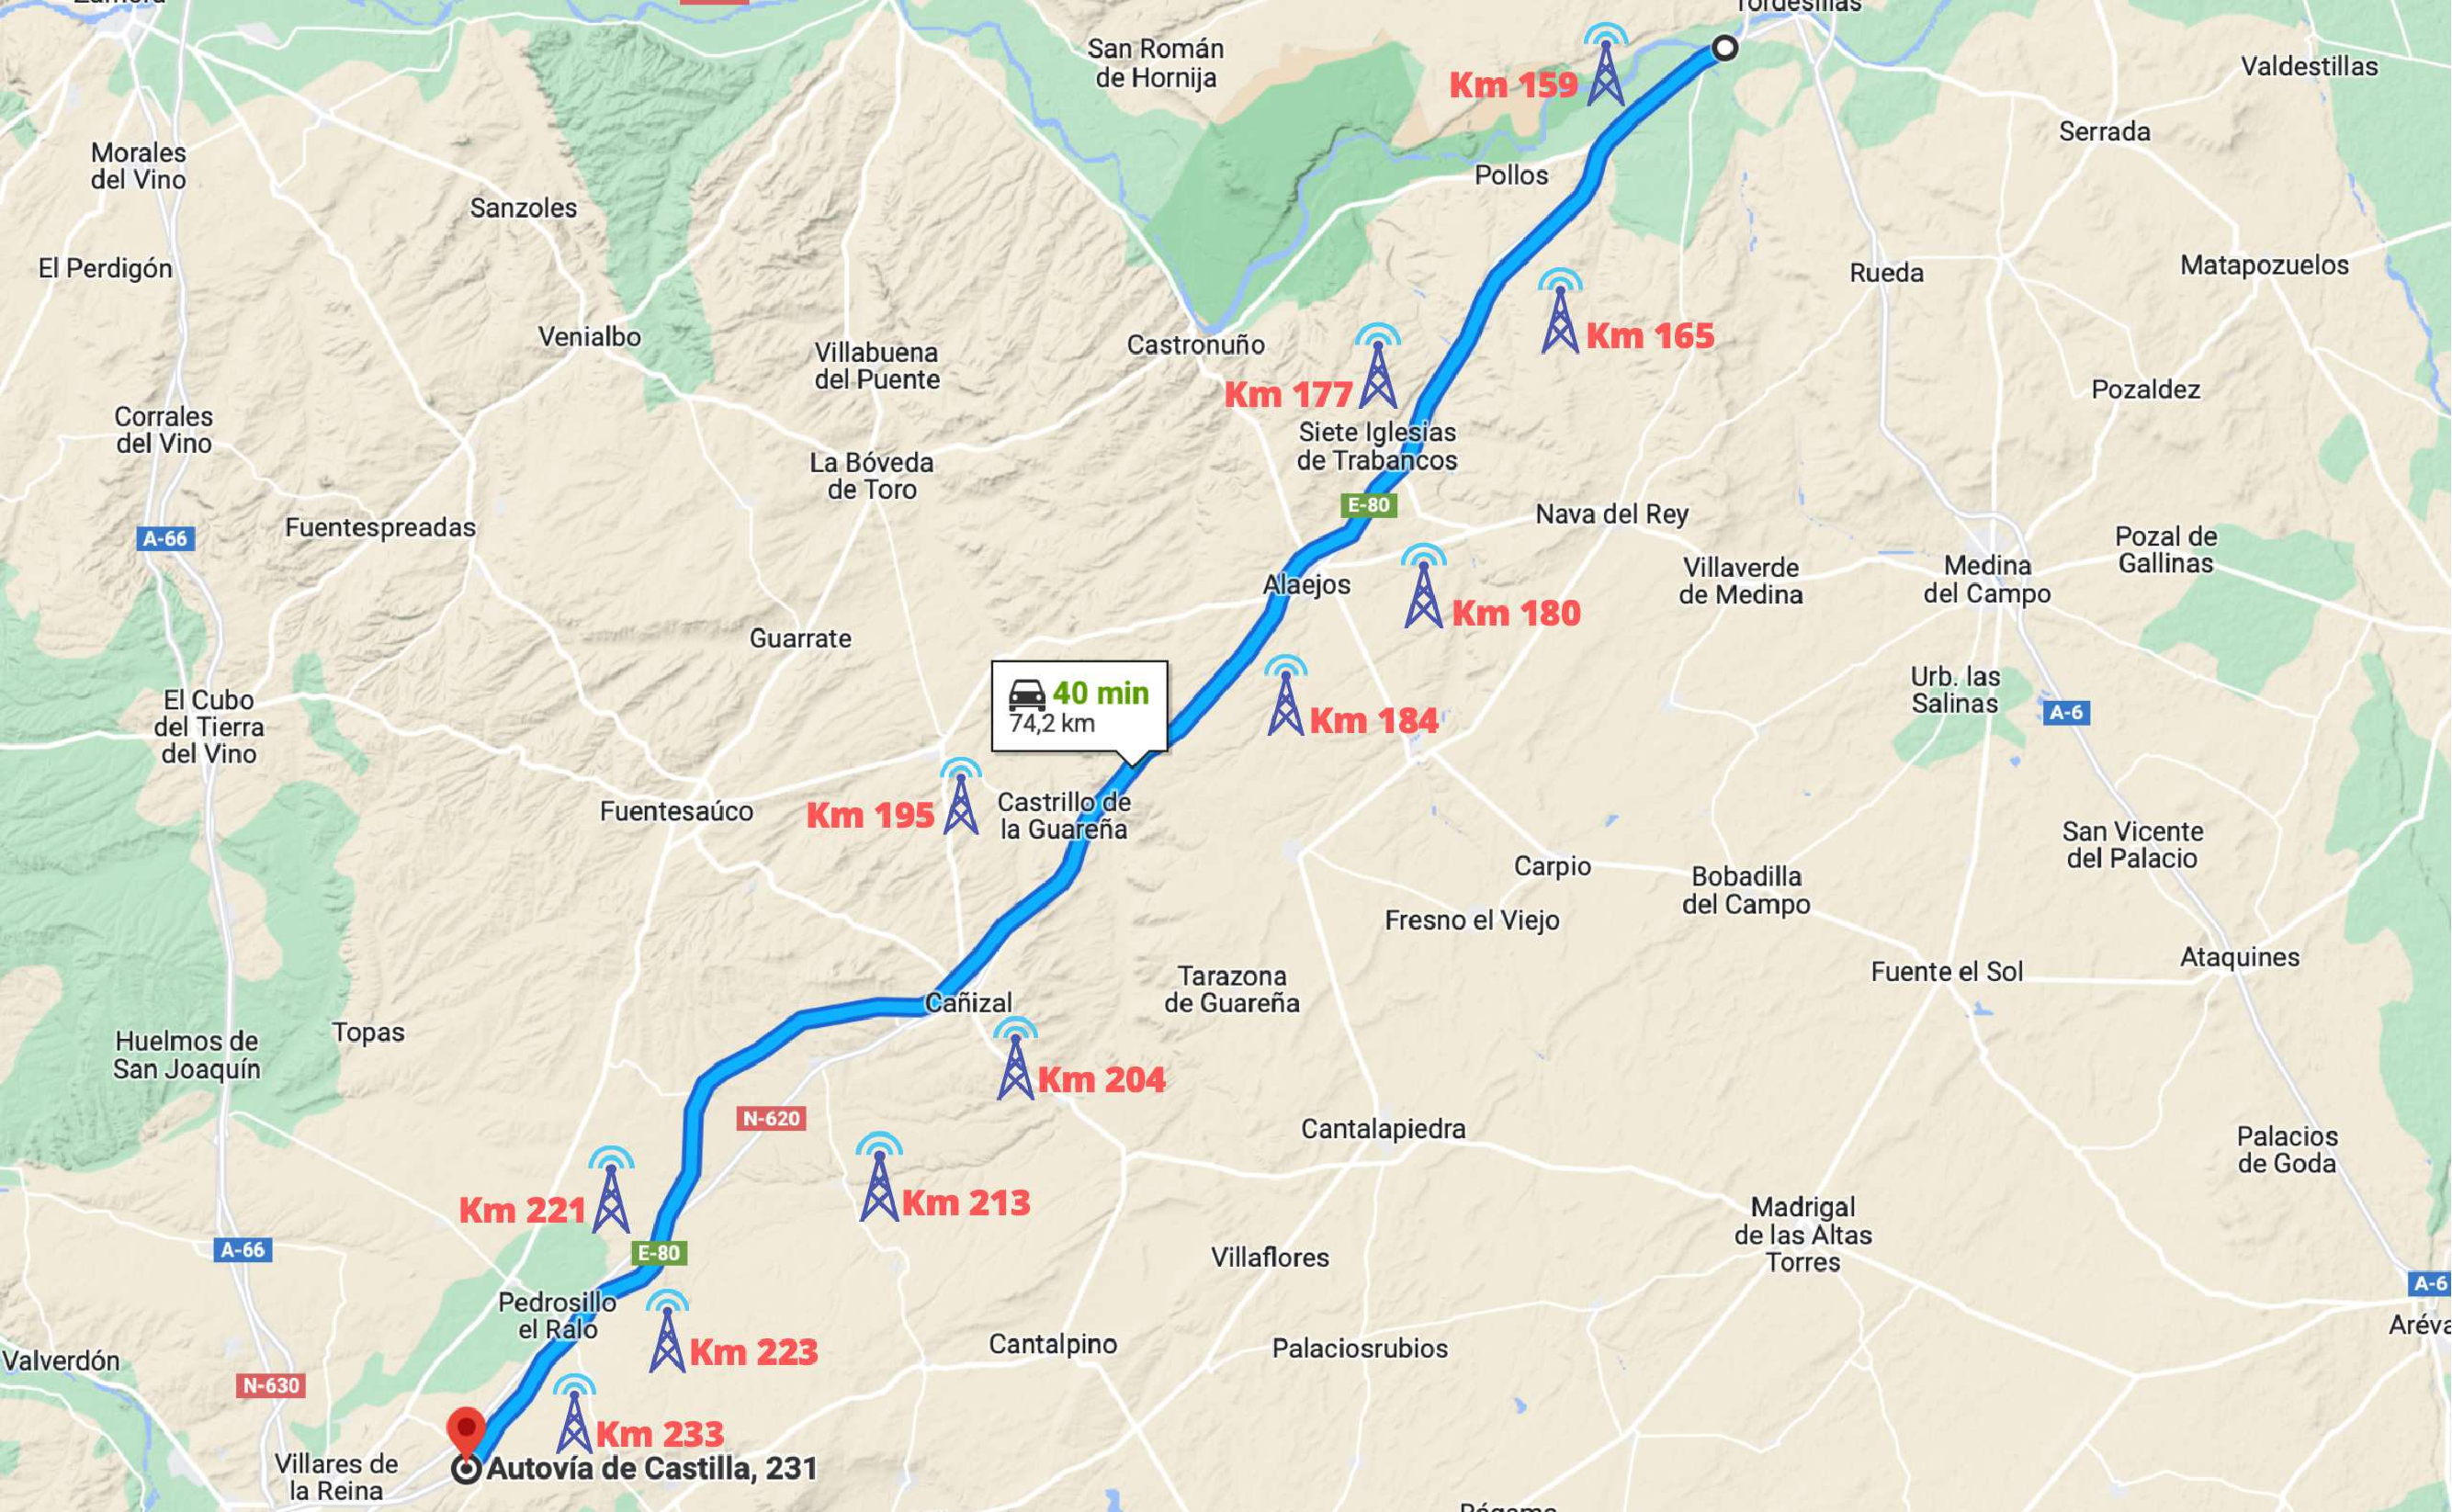
\includegraphics[width=\textwidth]{Imagenes/PlanteamientoInicial/torres_telefonia.pdf}
    \caption{Mapa de la autovía A-62 y las torres de comunicación existentes }
    \label{autovia}
\end{figure}

Queremos que un número elevado de coches pueda hacer uso de dicho servicio de manera ininterrumpida, es decir, que cada coche tenga capacidad suficiente para enviar el vídeo captado por la cámara durante todo el recorrido. Por eso, es necesario disponer de un ancho de banda de al menos varios Mbps, todo dependiendo de la calidad del vídeo que queramos ofrecer. \\

Prestando este servicio, los vehículos de los usuarios tendrán la capacidad de detectar las señales de tráfico aumentando así la seguridad vial, ya que así los vehículos pueden adaptar su velocidad y comportamiento en la carretera, lo que puede reducir el riesgo de accidentes y mejorar la seguridad en general. De igual forma, puede fomentar el cumplimiento de las normativas y regulaciones de tráfico, disminuir la cantidad de sanciones, o puede ayudar a optimizar el consumo de combustible y moderar las emisiones de gases contaminantes procedentes de dichos vehículos.\\

La seguridad en las carreteras es uno de los temas más importantes en el mundo actual. Una de las medidas para garantizar la seguridad es la señalización vial, la cual indica a los conductores las condiciones y normas de circulación. Sin embargo, a menudo las señales pueden ser difíciles de identificar debido a factores como su ubicación, desconocimiento de la misma o la distracción del conductor.\\

Para resolver este problema, se puede utilizar el aprendizaje automático para diseñar modelos capaces de detectar de manera precisa y eficiente las señales de tráfico. Estos modelos pueden ayudar a mejorar la seguridad en las carreteras permitiendo que los conductores reciban información clara y precisa en todo momento.\\

En este contexto, nuestra empresa ha sido encargada de diseñar e implementar un modelo de aprendizaje automático para la detección de señales de tráfico. Para eso, debemos utilizar técnicas avanzadas de procesamiento de imágenes. El objetivo final es contribuir a la seguridad en las carreteras y ofrecer soluciones innovadoras y eficaces.\\

Con el objetivo de poder prestar dicho servicio, se debe elegir qué modelo de inteligencia artificial se va a seleccionar para llevarlo a cabo. En el campo de la detección de objetos en imágenes y vídeos, existen varios modelos de aprendizaje automático que se pueden utilizar. Uno de los más avanzados y precisos es YOLO. Lo que le distingue de otros modelos es su capacidad para detectar múltiples objetos en una sola imagen de manera eficiente y precisa, utilizando redes neuronales convolucionales (CNN) y técnicas de filtrado de cajas delimitadoras. \\



\chapter{Solución}
	\section{Metodología del proyecto}
		Hacer un poco resumen de lo que se va a hacer y el planteamiento
	
	\section{Infraestructura}
		En primera instancia, se debe decidir cómo se quiere plantear la infraestructura de red, si vamos a construir nuestras propias torres, si vamos a funcionar como una operadora virtual, o si por el contrario, vamos a comprar a instalar nuestros propios equipos. En nuestro caso, nos hemos decantado por alquilar las torres de telecomunicaciones existentes, en las cuales vamos a instalar nuestros propios componentes. De esta manera, lograremos diseñar una red que cumple con compromisos económicos y, que a la vez, nos proporcionan cierto control en caso de averías o problemas.\\

Además, debemos conocer dónde se encuentran las torres de telecomunicaciones existentes. Existen varias páginas web a través de las cuales podemos conocer dicha información, como Infoantenas \url{https://geoportal.minetur.gob.es/VCTEL/vcne.do}, un servicio desarrollado por parte del Ministerio de Asuntos Económicos y Transformación Digital, o AntenasGSM \url{https://antenasgsm.com}. A través de dichas páginas hemos podido conocer la localización de las torres, mostradas en la figura \ref{autovia}.\\

Sin embargo, tras seleccionar el modelo de estación base y antena que vamos a utilizar (en función de sus distintas características técnicas) hemos propuesto un diseño de infraestructura, en la cual no va a ser necesario utilizar todas las torres de telecomunicaciones disponibles. Existen 11 torres desplegadas y utilizaremos 7 de ellas. En origen las distintas torres pertenecían a las propias empresas operadoras que prestan el propio servicio, o empresas filiales de las mismas. No obstante, la mayoría de ellas han vendido una gran cantidad de las torres a otras empresas, como pueden ser Cellnex Telecom, una empresa española, o American Tower Corporation, empresa estadounidense, ambas se dedican a la construcción y gestión de infraestructuras de telecomunicaciones \cite{elmundo2021}, \cite{heraldodiariodesoria2019}. Se estima que el alquiler de estas torres se encuentra en torno a los 4.000 y 20.000 euros en zonas urbanas, y 1.000 y 15.000 euros en zonas rurales, costo que habrá que tener en cuenta a la hora de presupuestar la infraestructura.\\

Para el diseño del proyecto se ha contactado con los principales distribuidores en España de estos componentes, como pueden ser Ericsson, Nokia, Kathrein o Moyano Telsa, con el objetivo de lograr una red lo más similar a lo que nos podemos encontrar en las grandes operadoras españolas. Sin embargo, ninguna de estas empresas nos ha respondido ni nos has facilitado un catálogo de sus productos, por ello, hemos procedido a diseñar la red con equipos de los cuales si hemos podido encontrar información. \\

En primer lugar, hemos seleccionado una estación base proporcionada por una empresa china llamada Baicells, una compañía fundada en 2014 con sede en cinco continentes que ofrece productos de tecnología inalámbrica 4G y 5G. El modelo concreto es el Nova846, este nos proporcionará una potencia de transmisión entre 0 y 37 dBm, una distancia máxima de 60km y una sensibilidad diferente en función del rango de distancias en el que se encuentra el usuario gracias a la modulación adaptativa.\\

\begin{table}[H]
\centering
\begin{tabular}{|c|c|c|}
\hline
\textbf{Esquema de modulación} & \textbf{RSRP {[}dBm{]}}            & \textbf{Distancia cubierta {[}km{]}} \\ \hline \hline
QPSK                           & -120 \textless RSRP \textless -110 & Entre 40 y 60                        \\ \hline
16 QAM                         & -110 \textless RSRP \textless -100 & Entre 10 y 40                        \\ \hline
64 QAM                         & -100 \textless RSRP \textless -85  & Entre 4 y 10                         \\ \hline
256 QAM                        & RSRP \textgreater -85              & Menor a 4                            \\ \hline
\end{tabular}
\caption{Cobertura en función de la modulación.}
\label{cobertura}
\end{table}

Dependiendo de la configuración se proporcionará un rendimiento u otro, en nuestro caso nos hemos decidido por la configuración 6. Esta nos brindará un rendimiento máximo en el enlace de subida, que nos interesa que sea máximo para que el mayor número de usuarios pueda enviar el vídeo en streaming. Lograremos tener las distintas capacidades mostradas para el enlace de \textit{downlink} y \textit{uplink}.\\

\begin{table}[H]
\centering
\begin{tabular}{|c||c|c|}
\hline
\textbf{Modulación} & \textit{\textbf{DownLink}} & \textit{\textbf{UpLink}} \\ \hline \hline
256 QAM             & 348 Mbps                   & 92 Mbps                  \\ \hline
64 QAM              & 264 Mbps                   & 70 Mbps                  \\ \hline
16 QAM              & 70 Mbps                    & 53 Mbps                  \\ \hline
QPSK                & 53 Mbps                    & 53 Mbps                  \\ \hline
\end{tabular}
\caption{Capacidades del enlace de bajada y de subida}
\label{capacidad}
\end{table}

La antena seleccionada es fabricada por la empresa irlandesa Alpha Wireless, una compañía fundada en 2006 dedicada a la fabricación de antenas. El modelo seleccionado es el AW3864-E-F, una antena sectorial de 4G que nos proporciona un ancho de haz de 65$\deg$ y una ganancia de 18 dB en las frecuencias de interés.\\

Con estos datos nos encontramos en disposición de simular la infraestructura, para ello hemos utilizado la herramienta de planificación y diseño de redes de telecomunicaciones Xirio-online. Una plataforma desarrollada una empresa española llamada Xirio, especializada en soluciones de ingeniería para telecomunicaciones. Con ésta se pueden crear mapas de cobertura y realizar simulaciones de propagación de señal con redes de telefonía móvil o televisión digital entre otras, así como evaluar del rendimiento de la red.\\

A través de un estudio de multicobertura e introduciendo todos los parámetros ya mencionados en la herramienta, hemos dispuesto las antenas a lo largo de tramo de autovía en las distintas ubicaciones en las que previamente localizamos las torres de telecomunicaciones. Como se puede apreciar en la figura \ref{xirio} teniendo en cuenta la cartografía del terreno, podremos cubrir la totalidad de la carretera a través de 7 estaciones base y 12 antenas. Asimismo, dado que no hemos logrado averiguar la altura exacta de cada una de las torres utilizadas, hemos supuesto una altura de 30 metros para todas ellas, ya que la altura media se encuentre en 15 y 50 metros.

\begin{figure}[H]
\centering
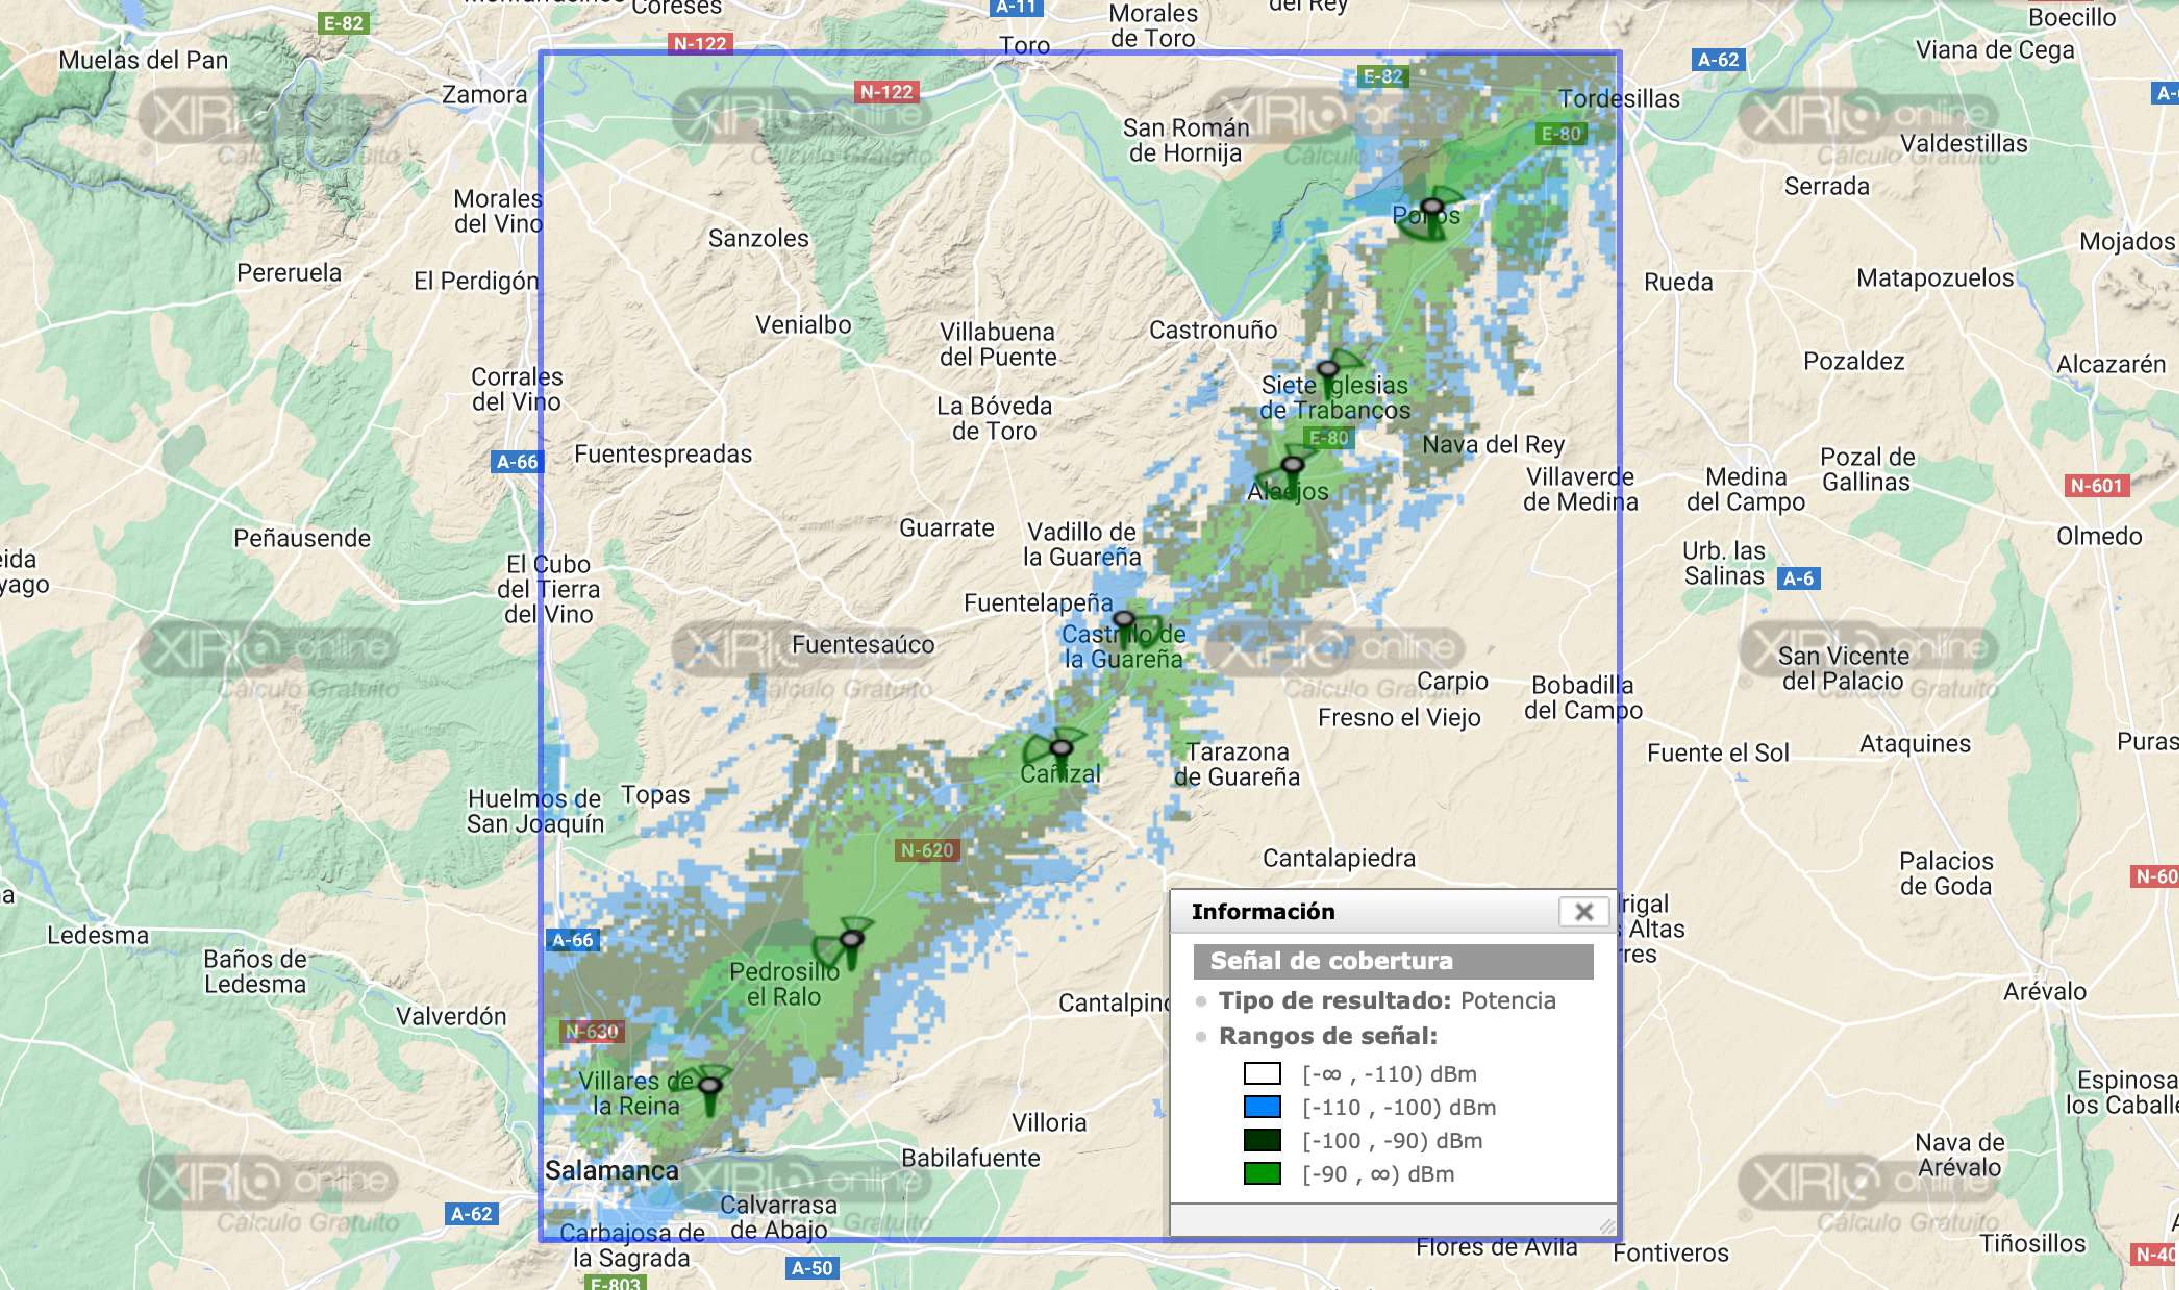
\includegraphics[width=\textwidth]{Imagenes/Solucion/xirio.pdf}
\caption{Distribución de la cobertura y estudio de cobertura}
\label{xirio}
\end{figure}

Un detalle muy importante del proyecto es conocer cuál es la cantidad de usuarios a la que se podrá prestar el servicio de detección de señales de tráfico. Tal y como hemos distribuido las antenas y estaciones base, en prácticamente todo el tramo  de autovía se proporciona una potencia suficiente como para que los usuarios operen a través de la modulación 256 QAM. De este modo, podremos calcular la cantidad de usuarios a la cual podremos prestar servicio en función de las distintas velocidades que nos podríamos encontrar.  Dividiendo la capacidad del enlace de subida entre la cantidad de Mbps necesarios para transmitir por cada usuario, podremos conocer el número de usuarios posible de manera simultánea, teniendo en cuenta además cuál es la distancia y fotogramas por segundo adecuados para poder detectar la señal con fiabilidad.

\begin{table}[H]
\centering
\begin{tabular}{|c|c|c|c|c|}
\hline
\textbf{Distancia} & \textbf{Velocidad} & \textbf{Frames/Sec} & \textbf{Mbps} & \textbf{Cantidad Usuarios} \\ \hline \hline
20 metros          & 80 km/h            & 12 f/s              & 2 Mbps        & 46 usuarios                \\ \hline
20 metros          & 100 km/h           & 15 f/s              & 2,5 Mbps      & 36 usuarios                \\ \hline
20 metros          & 120 km/h           & 18 f/s              & 3 Mbps        & 30 usuarios                \\ \hline
\end{tabular}
\caption{Cantidad de usuarios disponibles en función de la velocidad del vehículo }
\label{users}
\end{table}

La interconexión entre las estaciones base y el núcleo de la red 4G se establecerá utilizando una topología de estrella, donde el núcleo se situará en Madrid junto con el centro de operaciones (CTO). Esta elección permite centralizar la gestión completa del servicio en una ubicación, lo que brinda ventajas logísticas en caso de necesitar intervenciones. La elección de Madrid se basa en su ubicación geográfica estratégica y en la disponibilidad de abundantes recursos.\\

El core de la red 4G, esencial para proporcionar servicios de conectividad y gestionar el tráfico de datos, se implementará utilizando la solución Telrad BreezeWAY2020 de Telrad Networks. Telrad Networks, una empresa líder en el sector de las telecomunicaciones desde 1951, ofrece esta solución que tiene la capacidad de atender simultáneamente a 10.000 usuarios. Además, cuenta con una Arquitectura de Clúster Distribuido que permite un escalado gradual y prácticamente ilimitado en términos de capacidad y rendimiento a nivel de red.\\

El centro de operaciones se encargará de la detección de señales de tráfico utilizando modelos de inteligencia artificial, como YOLO v3. Dado el alto requerimiento computacional de este servicio, ha surgido el debate sobre si es más conveniente adquirir una gran cantidad de servidores o bien optar por servicios en la nube ofrecidos por grandes empresas tecnológicas como AWS (Amazon) o Azure (Microsoft).\\

En el contexto de los vehículos autónomos, se ha observado una tendencia creciente hacia la realización del cálculo computacional en el propio vehículo. Esto se debe a que delegar un mayor acceso y control externo aumenta los riesgos de seguridad. Por lo tanto, resulta más seguro realizar el procesamiento de datos en el vehículo mismo.\\

En línea con esta consideración, se ha decidido alquilar los servicios de AWS, ya que una inversión inicial significativa no sería viable a largo plazo, dado que en el futuro estos servicios podrían no utilizarse para este propósito.\\

El núcleo de nuestra red establece su conectividad a Internet mediante un enlace de conexión dedicado, el cual puede ser suministrado por un proveedor de servicios de Internet (ISP) o a través de una conexión de fibra óptica. Es fundamental que este enlace posea una velocidad y fiabilidad adecuadas para gestionar eficientemente el tráfico de datos generado por los usuarios de la red 4G.

		
	\section{Detección de señales de tráfico}
		Hablar de manera resumida y sencilla la forma en la que se va a implementar la deteccion de señales

\chapter{Normativa}

\chapter{Costes}

\chapter{Conclusiones}

\chapter{Anexo I: Infraestructura 4G}
	\section{Software}	
	\section{Componentes}
	\section{Infraestructura de la red}
		Para el proceso de creación de la red 4G, se usó el \textit{software} srsRAN, una implementación de código abierto de una red de acceso radio (RAN) que utiliza \textit{hardware} SDR. En nuestro caso, se ha utilizado una BladeRF 2.0 micro xA9 de Nuand con dos canales rx y tx MIMO.

Para ello, se siguieron los siguientes pasos:


\begin{enumerate}
\item Descarga de la última versión de \textbf{Ubuntu}, \textbf{22.04 LTS}.
\item Grabación de la ISO en un pincho a través de \textbf{UNetbootin} y posterior instalación de Linux en un ordenador sin sistema operativo (proporcionado por la empresa).
\item Instalación de los drivers de la \textit{Blade} siguiendo el manual de \textit{GitHub}:\\
 \url{https://github.com/Nuand/bladeRF/wiki/Getting-Started:-Linux}

\begin{lstlisting}
sudo add-apt-repository ppa:nuandllc/bladerf
sudo apt-get update
sudo apt-get install bladerf
\end{lstlisting}

\item Conexión de la Blade: Las antenas se deben conectar en los puertos tx1 y rx1 (configuración por defecto, sin embargo se podrían conectar a tx2 y rx2 haciendo los cambios correspondientes en los ficheros de configuración) con un grado de 90º entre ellas para evitar el efecto de \textit{crosstalk}, como se muestra en la figura \ref{blade}. La Blade se debe conectar a un puerto USB 3.0 que presente el ordenador ya que en un puerto USB 2.0 no se detectaría correctamente.\\

\begin{figure}[H]
	\centering
	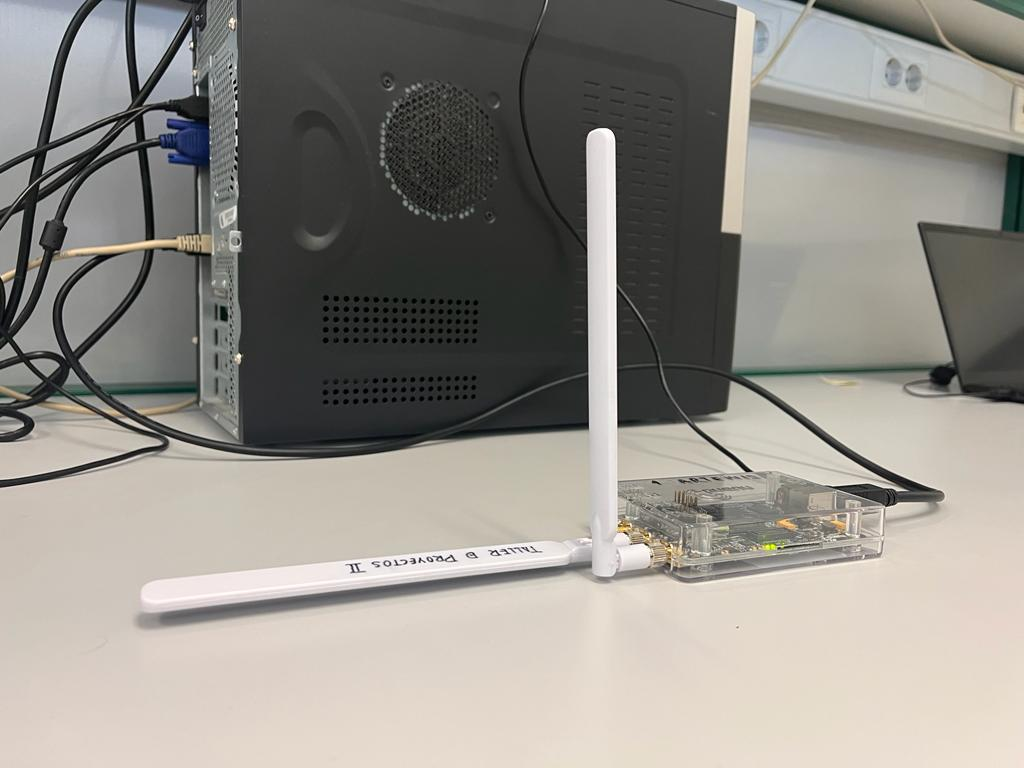
\includegraphics[width=\textwidth]{Imagenes/AnexoI_Manual/RED/blade.jpeg}
	\caption{Dataset descargado con los ficheros TXT}
	\label{blade}
\end{figure}

\item Instalación de \textbf{srsran} siguiendo el manual de GitHub y las librerías \textbf{boost} y \textbf{libboost}:\\
\url{https://docs.srsran.com/projects/4g/en/latest/general/source/1_installation.html}\\
\url{https://docs.srsran.com/projects/4g/en/latest/getting_started.html}

\begin{lstlisting}
git clone https://github.com/srsRAN/srsRAN_4G.git
cd srsRAN_4G
mkdir build
cd build
cmake ../
make
make test
sudo make install
srsran_4g_install_configs.sh user
\end{lstlisting}

\item Modificación de los archivos de configuración que se encuentran en la ruta \textit{root/.config/srsran/}. Los cambios se deben hacer como superusuario:
\begin{itemize}
	\item epc.conf: contiene la configuración específica de un controlador de paquetes Evolved Packet Core (EPC) en una arquitectura de red LTE 
	\item enb.conf: cotiene la configuración específica de un nodo de banda base (eNodeB).
	\item user_db.csv: que contiene una base de datos de usuarios en formato tabular.
\end{itemize}

En el archivo \textbf{enb.conf} se cambiaron los valores de \textbf{MCC} y \textbf{MNC} que están disponibles en las hojas de datos de las SIMs (y en la propia tarjeta SIM), y se establecieron sus valores correspondientes (\textbf{901-70}) para que correspondan con el IMSI. También se modificó el valor de la frecuencia central. cambiando el valor de \textbf{dl_earfcn}, para ello se utilizó \cite{earn}, estableciéndolo este valor 3050, lo que corresponde a un valor de frecuencia central \textit{downlink} de 2650.  Por último, se estableció el ancho de banda en 5MHz cambiando el valor de \textbf{n_prb} a \textbf{25}. Para mejorar el alcance de la red, se aumentó la ganancia de transmisor, cambiando el valor de \textbf{tx_gain} a 90.

En el archivo \textbf{epc.conf} se modificaron los valores de \textbf{MCC} y \textbf{MNC} (igual que en el caso anterior) y se añadieron los nombres de la red con:
\begin{lstlisting}
    full_net_name= NOMBRE
    short_net_name= NOMBRE
\end{lstlisting}

En el archivo \textbf{user_db.csv} se creó un usuario nuevo con la siguiente información:
\begin{lstlisting}
    nombre, mil (Auth), IMSI (aparece en las hojas de las sims),
    KEY (aparece en las hojas de las sims), opc,
    OPC(aparece en las hojas de las sims), 9000,
    sqn (poner todo a ceros, aunque cada vez que se levanta la red cambia automáticamente),
    7 (QCI), dynamic (IP_alloc)
\end{lstlisting}

\item Ahora que tenemos conectividad entre el enb y el epc, necesitamos que estos la tengan para el exterior, por lo que necesitamos configurar el ordenador (que ejecuta el núcleo) para que reencamine los paquetes a través de la interfaz de red. Para eso ejecutamos el siguiente comando.

\begin{lstlisting}
    srepc_if_masq.sh enp0s25
\end{lstlisting}

\item Una vez está la red configurada, es hora de levantarla, ejecutamos:
\begin{lstlisting}
    srsepc epc.conf
    srsenb enb.conf
\end{lstlisting}

\item Una vez obtenida la conexión a internet con la red 4G, nos bajamos los ficheros \textit{python} de control del coche para crear el servidor \textit{cloud} e instalamos el servidor \textbf{MQTT Mosquitto}, diseñado para facilitar la comunicación entre dispositivos (en nuestro caso la SDR y el coche) itercambiando mensajes MQTT. Este servidor facilita la integración del proyecto, facilitando el monitoreo y control remoto del coche durante su funcionamiento.
Para su instalación en el ordenador (que actuará como servidor), se ejecutan los siguientes comandos:

\begin{lstlisting}
	sudo apt-get update
	sudo apt-get install mosquitto
\end{lstlisting}

\item Modificamos el fichero de configuración /etc/mosquitto/mosquitto.conf con las siguientes líneas:
\begin{lstlisting}
	persistence true
	persistence_location /var/lib/mosquitto/
	allow_anonymous true
	listener 1883 10.0.128.176
	bind_interface enp0s25
	log_type information
	log_type warning
	log_type error
\end{lstlisting}

\item Una vez configurados los ficheros, reiniciamos el servicio mosquitto para que se apliquen los cambios:
\begin{lstlisting}
	sudo systemctl restart mosquitto
\end{lstlisting}

\item Para instalar el servicio en el móvil (que actuará como cliente) usamos la aplicación MyMQTT. Para comprobar el tránsito de mensajes que el coche envía nos suscribimos a los tópicos básicos que se especifican en el manual de usuario del coche. Para ello, habrá que poner el ID del vehículo y el tópico al que nos queramos suscribir (Ver figura \ref{fig:mosq1}). Si la comunicación es exitosa, se debería observar algo similar a la imagen \ref{fig:mosq3}:

 \begin{figure}[H]
    \centering
    \subfloat[Suscripciones a los tópicos desde el móvil\label{fig:mosq1}]{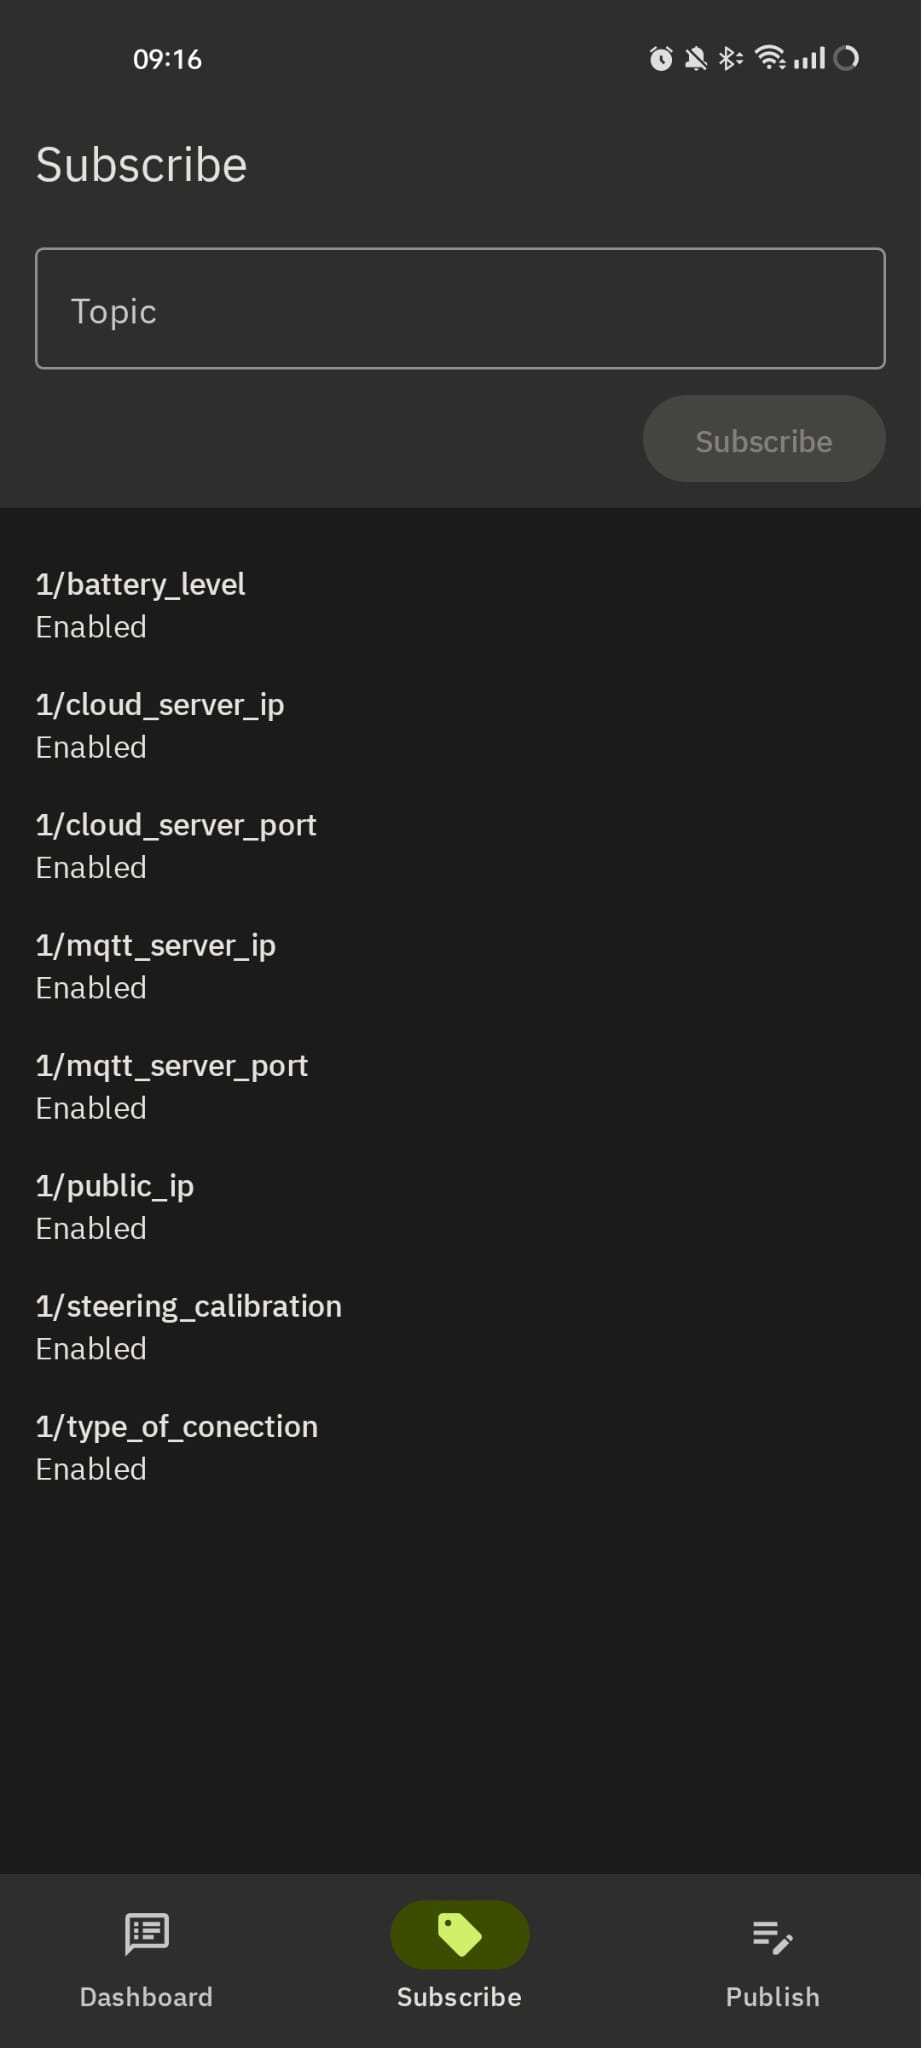
\includegraphics[width=0.4\textwidth]{Imagenes/Rendimiento/mosquitto1.jpeg}}
    \hspace{0.5cm}
    \subfloat[Información mostrada al iniciar la conexión\label{fig:mosq3}]{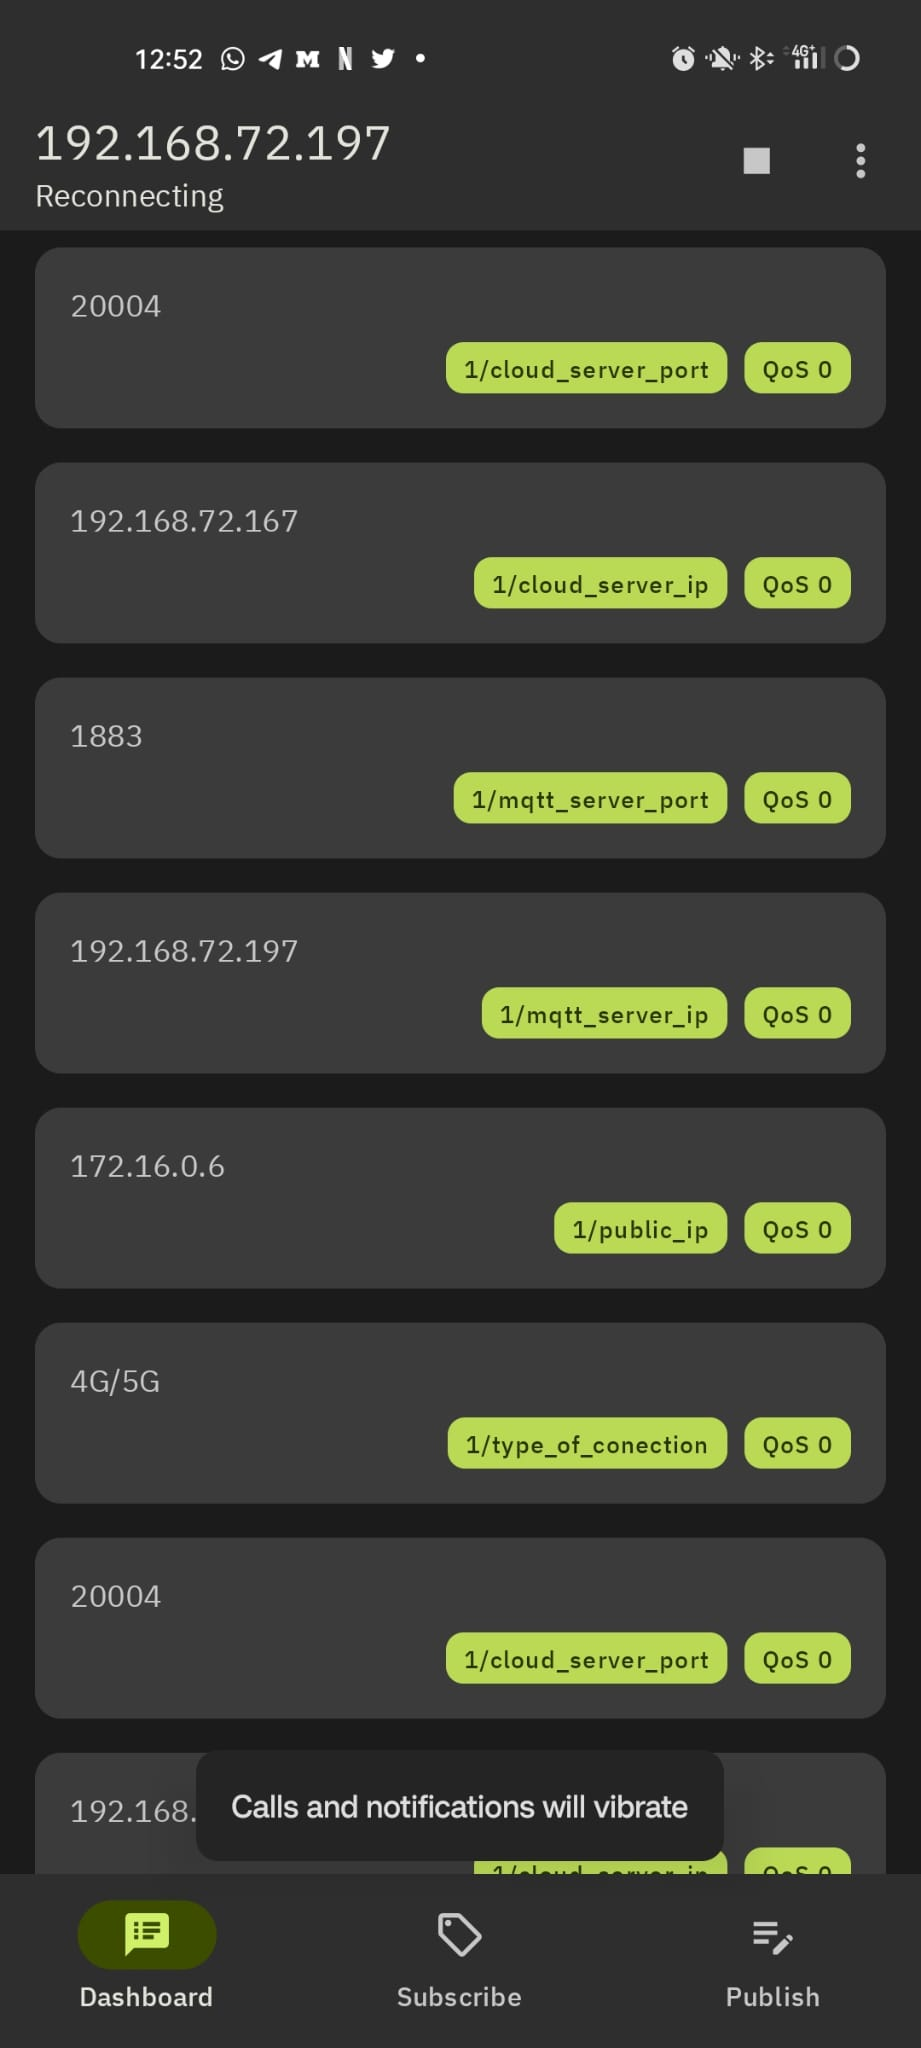
\includegraphics[width=0.4\textwidth]{Imagenes/Rendimiento/mosquitto3.jpeg}}
    \caption{Capturas de pantalla de la aplicación móvil MyMQTT para cliente suscrito}
\end{figure}


\item Tras configurar tanto el servidor como el cliente mosquitto, lanzamos el servicio y comprobamos su estado usando los comandos:
\begin{lstlisting}
	sudo systemctl start mosquitto
	sudo systemctl status mosquitto
\end{lstlisting}


\item Para comunicarnos con el coche, publicaremos los tópicos que se indican en el manual de configuración del coche, como podemos ver en la imagen \ref{mosquitto2}:

 \begin{figure}[H]
    \centering
    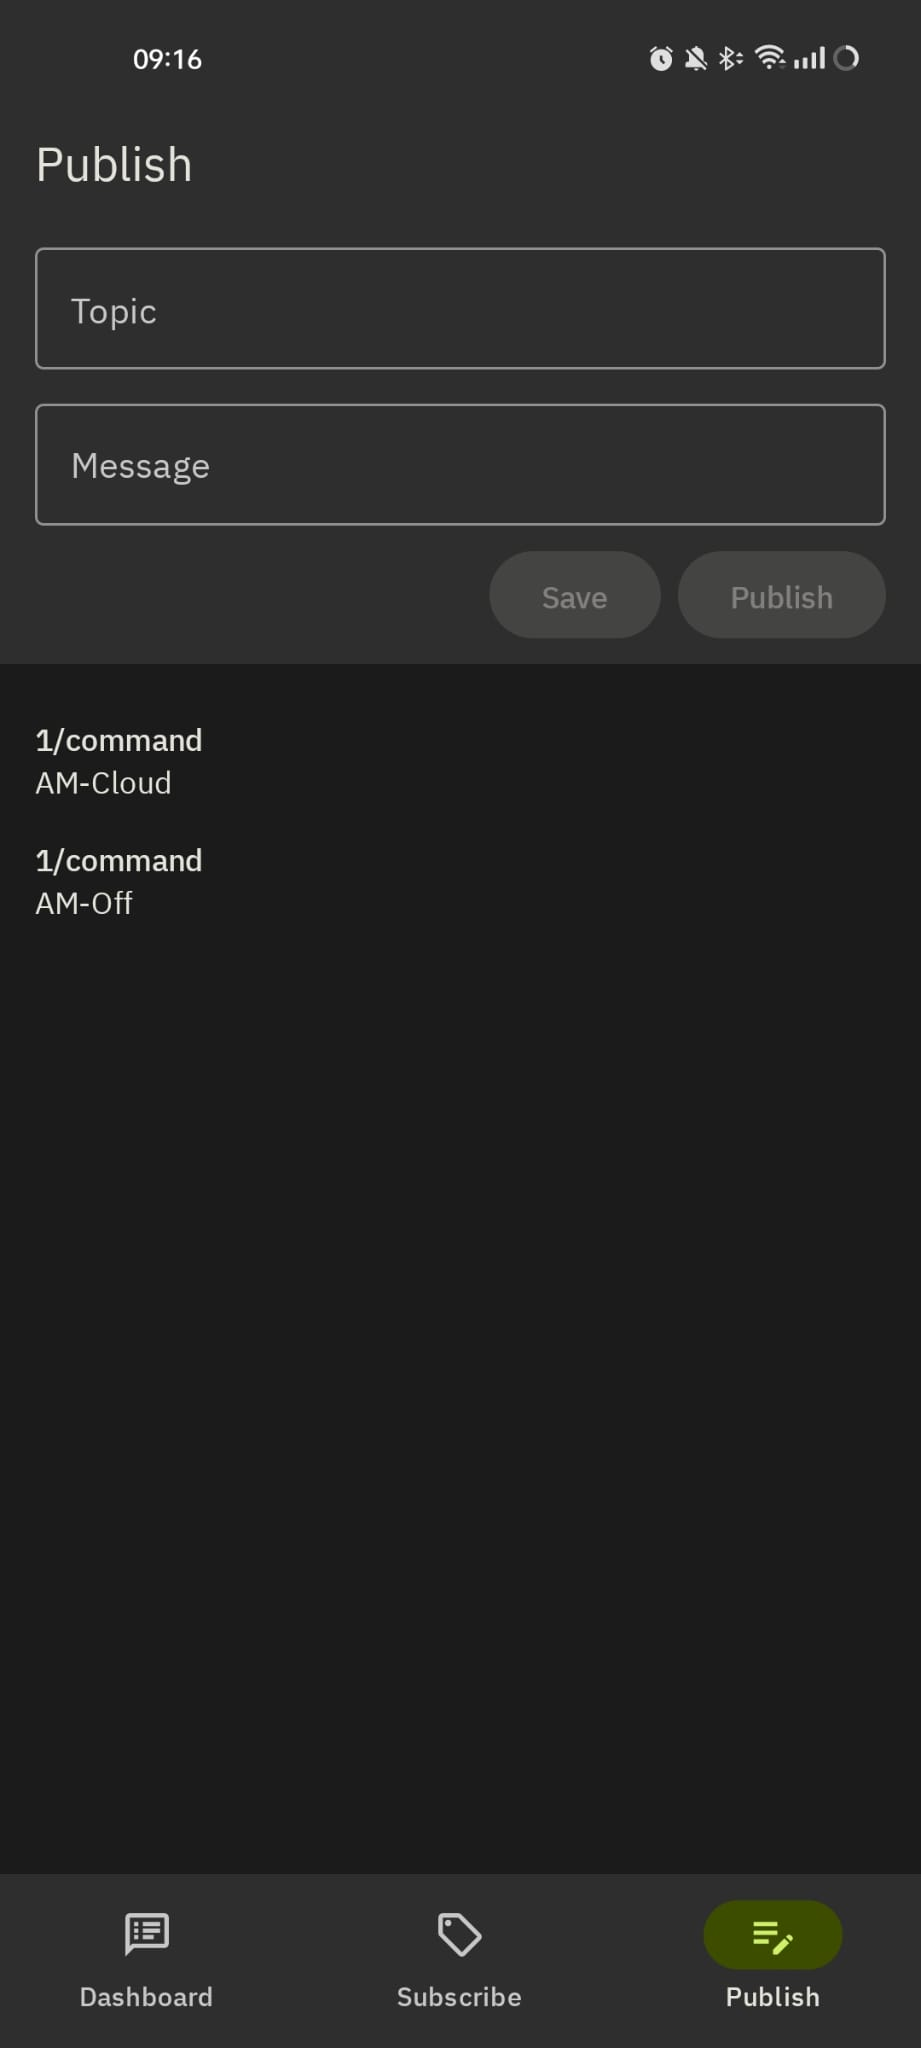
\includegraphics[width=0.35\textwidth]{Imagenes/Rendimiento/mosquitto2.jpeg}
    \caption{Publicación de comandos desde el móvil}
    \label{mosquitto2}
\end{figure}

\end{enumerate}

	
\chapter{Anexo II: Detección de señales de tráfico}
	\section{Modelos de IA}	
	\section{Identificación de imágenes}
	
\chapter{Anexo III: Normativa}

\chapter{Referencias}

\end{document}